\documentclass{article}
\usepackage[utf8]{inputenc}

\usepackage{ifxetex}
\ifxetex
  \usepackage{fontspec}
\else
  \usepackage[T1]{fontenc}
  \usepackage[utf8]{inputenc}
  \usepackage{lmodern}
\fi

\title{Reporte de Actividad 2}
\author{Roberto Benard Orci}
\date{06/02/2018}

\begin{document}
\maketitle

\section{Introducción}

En esta actividad se nos introdujo a Jupyter Notebook como entorno de programación, y con la ayuda de un ejemplo, exploramos las diferentes cosas que podíamos hacer con el lenguaje de programación Python. Después de terminar el ejemplo, se nos pidió realizar ciertas actividades adicionales para practicar lo que aprendimos con el ejemplo.

\section{Resumen}

Al comparar la forma de programación que usamos en Python, a través de Jupyter notebook, con la forma en la que programamos en FORTRAN, puedo decir que Python no se sintió muy diferente a FORTRAN, se sentía como si mezclara la terminal con el archivo de texto donde escribía el código, lo cual me pareció muy conveniente. 

En esta sesión practicamos distintos comandos de Python en Jupyter notebook, vimos que funciones podíamos usar para analizar una gran lista de datos y graficamos estos datos para compararlos y hacer conclusiones al respecto.

\subsection{Bibliotecas}

Antes que nada, tenemos que cargar a la memoria de trabajo de Python diferentes bibliotecas. Las bibliotecas son paquetes que te permitirán usar distintas funciones.
En nuestro caso, cargamos 3 bibliotecas: pandas, NumPy y matplotlib.pyplot.

\begin{center}
	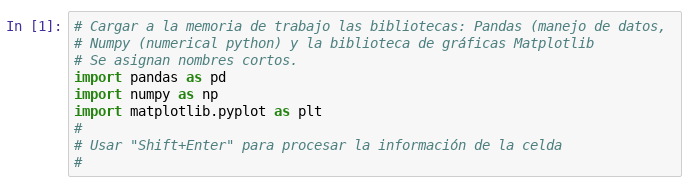
\includegraphics[width=12cm]{Act2bibliotecas.png}
    
    Bibliotecas
\end{center}
\vspace{0.3cm}

\subsubsection{Pandas}

Pandas es un paquete de Python que proporciona estructuras de datos rápidas, flexibles y expresivas diseñadas para que el trabajo con datos "relacionales" o "etiquetados" sea fácil e intuitivo.

\subsubsection{NumPy}

NumPy es el paquete fundamental para la programación científica con Python. Su uso principal es el de un contenedor multidimensional eficiente de datos genéricos.

\subsubsection{Matplotlib.pyplot}

Matplotlib es una biblioteca de bosquejo 2D de Python que produce figuras en una variedad de formatos impresos y entornos interactivos en todas las plataformas.
Matplotlib intenta hacer las cosas fáciles. Se pueden generar gráficos, histogramas, espectros de potencia, gráficos de barras, diagramas de errores, diagramas de dispersión, etc.

\begin{center}
	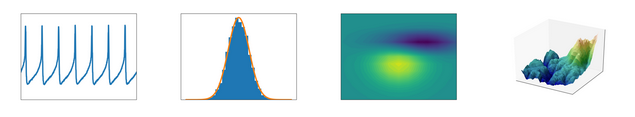
\includegraphics[width=12cm]{Act2Matplotlib.png}
    
    Graficas
\end{center}
\vspace{0.3cm}

\subsection{Lectura de un archivo}

Después de cargar las bibliotecas descargamos un archivo con los datos que use usaran para practicar diferentes funciones, para esto entramos a $http://smn1.conagua.gob.mx/emas/$ en donde escoges un estado, luego un municipio para ver diferentes datos del clima en esa región en la última semana (aproximadamente).

Luego utilizas la función para leer el archivo después de los primeros 4 renglones (ya que en estos no hay datos, solo el encabezado del archivo), y los separa por más de un espacio entre cada columna, para efectos estéticos del arreglo.

\subsection{Funciones}

Posteriormente utilizamos varias funciones para organizar los datos y ver distintas características de las columnas, como los tipos de datos que son, el número de datos, su promedio, desviación estándar, mínimo, máximo, los cuartiles, etc.
También utilizamos una función para unir las columnas de la fecha y la hora en una sola para hacer más sencillo el crear graficas.

\subsection{Graficas}

No fue muy difícil ver lo que se necesitaba para hacer una gráfica, a estas siempre incluimos 4 comandos, uno para nombrar la gráfica, otro para nombrar el eje $y$, otro para que la gráfica tuviera una cuadricula, y la más importante, para que se mostrara la gráfica. Pero había uno o a veces 2 renglones que siempre cambiaban o se modificaban, este dictaba que era lo que se graficaba, que columna, y en este podías personalizar su color, si se graficaban 2 columnas, o incluso, si se usaba otra columna para el eje vertical, en otras palabras, graficar una o más columnas en función de otra. 

\subsection{Actividades adicionales}

Después de haber copiado los ejemplos de las gráficas y deducir para que servía cada comando intente hacer estas \textit{actividades adicionales} por mi cuenta. Varias eran prácticamente idénticas a los ejemplos, pero intente practicarlas y moverles ciertas cosas.

\subsubsection{I}
\textit{Crear una gráfica que muestre la rapidez de los vientos y la rapidez de las ráfagas, como funciones del tiempo. ¿Cuáles son las horas del día con más viento?.}

\begin{center}
\begin{figure}[h]
\centering
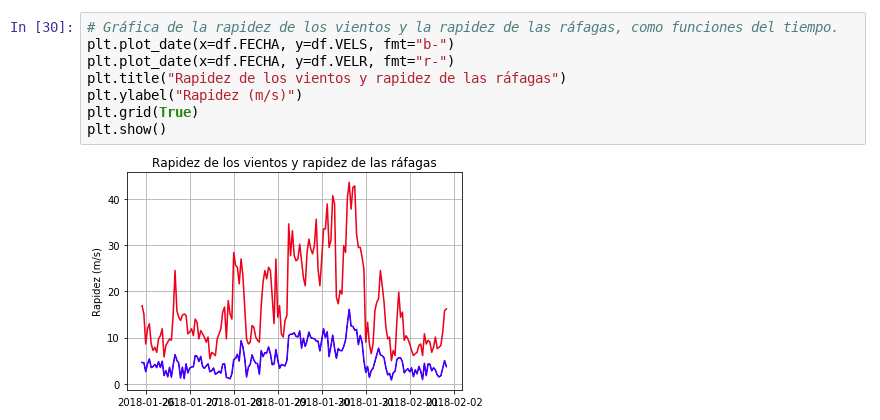
\includegraphics[width=12cm]{Act2i.png}
\end{figure}
    Rapidez de los vientos y rapidez de las ráfagas
\end{center}

Para esta primera actividad simplemente cree un $df1$ en el cual estuvieran las columnas de la rapidez de los vientos y la rapidez de las ráfagas. Las horas del día con más viento parecen ser las 3 y las 4 de la tarde.

\subsubsection{II}
\textit{Crear una gráfica con la dirección de los vientos como función del tiempo y comentar sobre los vientos dominantes en el sitio de estudio.}

\begin{center}
	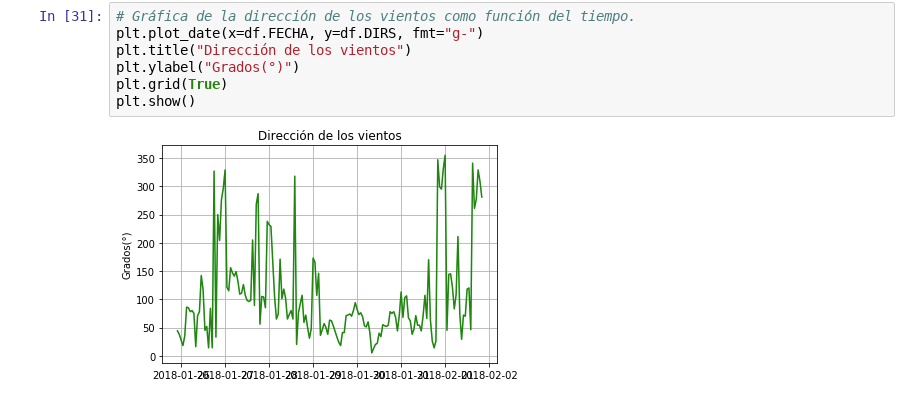
\includegraphics[width=12cm]{Act2ii.png}
    
    Dirección de los vientos
\end{center}
\vspace{0.3cm}

A pesar de que la dirección de los vientos parece ser muy dispersa, estos tienen una dirección entre 100 y 110 grados en promedio.

\subsubsection{III}
\textit{Muestre el comportamiento de la Radiación Solar como función del tiempo. ¿Que puedes comentar?} 

\begin{center}
	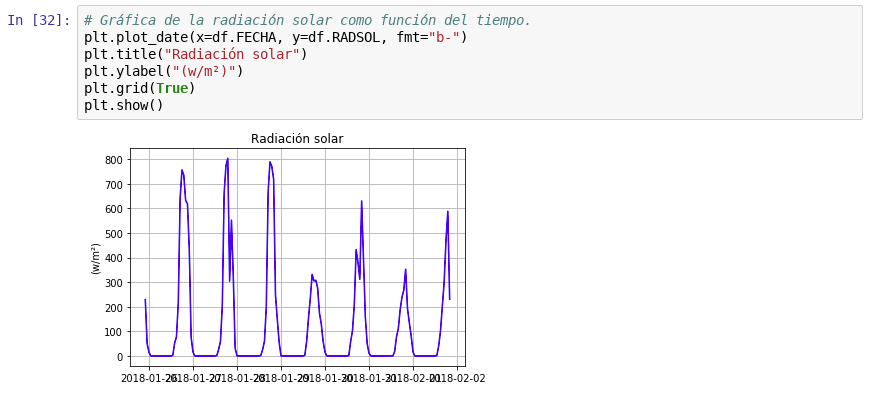
\includegraphics[width=12cm]{Act2iii.png}
    
    Radiación Solar
\end{center}
\vspace{0.3cm}

Que la es muy distintivo el nivel de radiación solar que recibe la región en el día a comparación de la noche, y que parece que en los últimos días del mes de enero esa región recibió más radiación que al inicio del mes de febrero.

\subsubsection{IV}
\textit{¿Cuál es el lapso de temperatura diaria? (Diferencia entre la temperatura máxima y la mínima).} 

\begin{center}
	\includegraphics[width=12cm]{Act2iv.png}
    
    Diferencia de temperatura
\end{center}
\vspace{0.3cm}

La diferencia es de 18.9 grados Celsius, la mínima siendo 8.5 y la máxima 27.4. 

\subsubsection{V}
\textit{¿Puedes comentar sobre la relación entre la temperatura y la humedad relativa?}

\begin{center}
	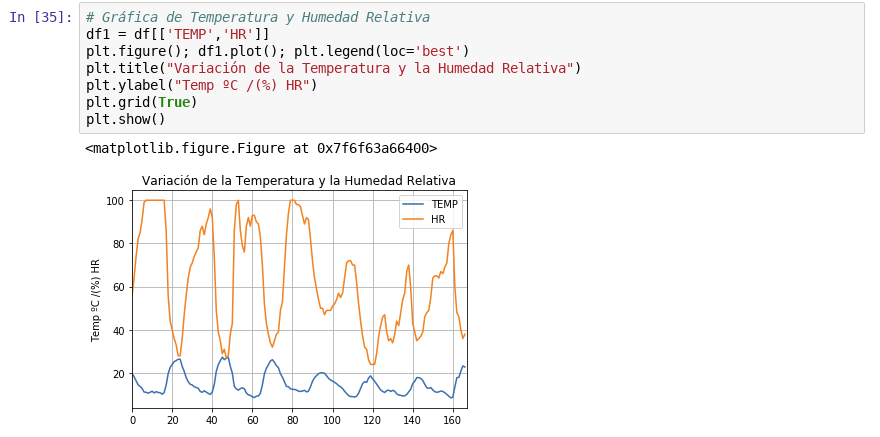
\includegraphics[width=12cm]{Act2v.png}
    
    Temperatura y humedad relativa
\end{center}
\vspace{0.3cm}

Son inversamente proporcionales, cuando una disminuye la otra aumenta.

\subsubsection{VI}
\textit{Realiza el análisis exploratorio de datos, que resuma el sitio estudiado (Usar la función describe() sobre tu data frame.} 

\begin{center}
	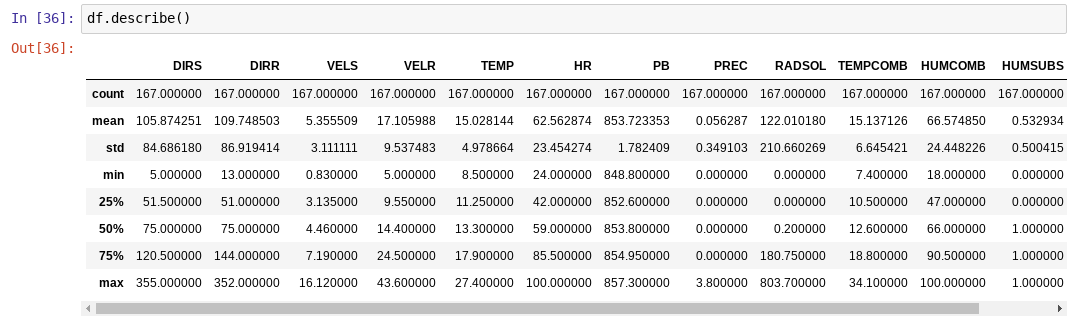
\includegraphics[width=12cm]{Act2vi.png}
    
    Ánalisis de datos
\end{center}
\vspace{0.3cm}

Esta función parece ser muy útil a la hora de realizar un análisis estadístico de un conjunto de datos, ya que te da muchos datos con los que puedes generar diferentes conclusiones, y con la inclusión de graficas uno puede tener una gran herramienta para estudiar conjuntos de datos.

\section{Bilbiografía}

\begin{verbatim}
(n.d.). Retrieved February 03, 2018, from http://smn1.conagua.gob.mx/emas/ 
\end{verbatim}
%http://smn1.conagua.gob.mx/emas/

\begin{verbatim}
Pandas: powerful Python data analysis toolkit¶. (n.d.). Retrieved February 03, 2018, 
from https://pandas.pydata.org/pandas-docs/stable/index.html 
\end{verbatim}
%https://pandas.pydata.org/pandas-docs/stable/index.html

\begin{verbatim}
Introduction. (n.d.). Retrieved February 03, 2018, from https://matplotlib.org/ 
\end{verbatim}
%https://matplotlib.org/

\begin{verbatim}
NumPy¶. (n.d.). Retrieved February 03, 2018, from http://www.numpy.org/ 
\end{verbatim}
%http://www.numpy.org/

\section{Apéndice}

 

    1.-¿Cuál es tu primera impresión de Jupyter Notebook?
    
    \vspace{0.3cm}
    Como mencione al principio en el resumen, me dio la impresión de una terminal combinada con un archivo de texto de código, eso me agrado mucho, se siente más fácil trabajar de esa manera.
    \vspace{0.3cm}
    
\noindent 2.-¿Se te dificultó leer código en Python?
    
    \vspace{0.3cm}
    Un poco, pero eso es de esperarse ya que es un lenguaje nuevo para mí. Recordando la primera vez que use FORTRAN, me parecía imposible hacer algo, y no entendía muy bien lo que hacía, pero después de un año de programar en FORTRAN me siento muy cómodo al usarlo. Se que con Python no será muy diferente, lo único que necesito es tiempo y práctica.
    \vspace{0.3cm}
    
\noindent    3.-¿En base a tu experiencia de programación en Fortran, que te parece el entorno de trabajar en Python?
    
    \vspace{0.3cm}
    Me pareció un poco menos riguroso, lo único que diría que no me gusto es que a la hora de cometer un error no tengo idea de que hice mal y siento que FORTRAN hace un mejor trabajo en señalar donde se encuentra el error.
    \vspace{0.3cm}
    
\noindent    4.-A diferencia de Fortran, ahora se producen las gráficas utilizando la biblioteca Matplotlib. ¿Cómo fue tu experiencia?. 
    
    \vspace{0.3cm}
    Esto fue algo que me gustó mucho de Python, su habilidad de cargar distintos paquetes de funciones (bibliotecas) para el uso que se le vaya a dar al programa, uno de los que usamos fue Matplotlib y, al ver los diferentes tipos de graficas que se pueden generar, estoy seguro de que será una herramienta muy útil.
    \vspace{0.3cm}
    
\noindent    5.-En general, ¿qué te pereció el entorno de trabajo en Python? 
    
    \vspace{0.3cm}
    En este momento siento que el entorno de trabajo es más relajado en FORTRAN, pero, como mencione, esto probablemente se deba a que no he usado Python tanto como FORTRAN, con el tiempo es probable que cambie de opinión.
    \vspace{0.3cm}
    
\noindent    6.-¿Qué opinas de la actividad? ¿Estuvo compleja? ¿Mucho material nuevo? ¿Que le faltó o que le sobró? ¿Qué modificarías para mejorar? 
    
    \vspace{0.3cm}
    Agregaría otro archivo con los comandos más básicos de Python, y más ejemplos con pequeños cambios para hacer énfasis en que comando o función hace que cosa. Empezando con el ejemplo más básico he ir subiendo de ahí.
    \vspace{0.3cm}
    
\noindent    7.-¿Comentarios adicionales que desees compartir?
    
    \vspace{0.3cm}
    Ninguno. 
    \vspace{0.3cm}

\end{document}